The Silicon Photomultiplier (SiPM) are a kind of photosensor, based on semiconductor materials, developed in recent years. They are replacing progresively conventional PMTs in many experiments and applications. They archieve outstading photon-counting capabilities with high photodetection efficiency comparing to PMT and a similar gain. They have conveninent characteristics as insensitiveness to magnetic fields, low operating voltage and compactness. The main problem with the SiPMs are their high dark count rate (between $100~\kilo\hertz$ and $1~\mega\hertz$)

The SiPM is formed by a matrix of APDs conected in parallel which are photodiodes operating in Geiger mode. A scheme of an APD is shown in Figure \ref{fig:SchemeAPD}. SiPM are based on p-n junctions\footnote{A p-n junction is a junction of a p+ and n+ layer, which are a tetravalent material doped with a trivalent or pentavalent material respectively, creating interesting sublevels in the forbidden energy gap.} made with special techniques to archieve a good contact between both surfaces.

\begin{figure}[htbp]
\centering
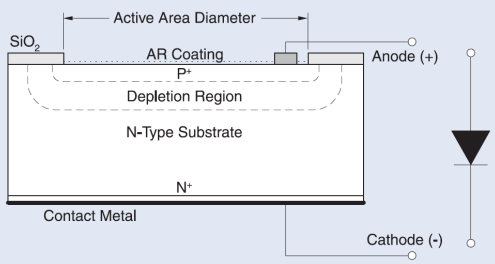
\includegraphics[scale=0.6]{3DesignPrinciples/32Tritium_detector/APD_scheme.png}
\caption{Scheme of a APD and electrical symbol used.\label{fig:SchemeAPD}~\cite{OSI}}
\end{figure}
 

The voltage at which the SiPM starts operating in geiger mode is called the breakdown voltage, $V_ {BR}$. At lower voltages SiPM works in proportional mode in which the signal of the pixel is proportional to the energy deposited the SIPM gain is lower in this state. The measurement of the breakdown voltage is one of the most important parametes to characterize the SiPM and its experimental measurements is described in section \ref{sec:CharacterizationSiPM}.

These APDs, called pixels when they are part of a SiPM, are connected in parallel and the sum of all of them is read. The output signal of the pixels are quite similar regardless of the energy deposited, with some difference because of the uncertainty due to the SiPM manufacturing process and the statistical nature of the detection process. In this way, the energy deposited in each APD is not known but the charge of the output signal when n photons are simultaneously detected is n times the charge of a single photon, as can be seen in Figure \ref{fig:PulsesOfSiPM}. Due to this property, the number of detected photons is linearly proportional to the area of the output signal and, after a correct calibration of SiPMs, shown in section \ref{sec:CharacterizationSiPM}, these can be known. In this way, the linearity of the output signal the SiPM and the deposited energy by the tritium event is recovered.

\begin{figure}[htbp]
\centering
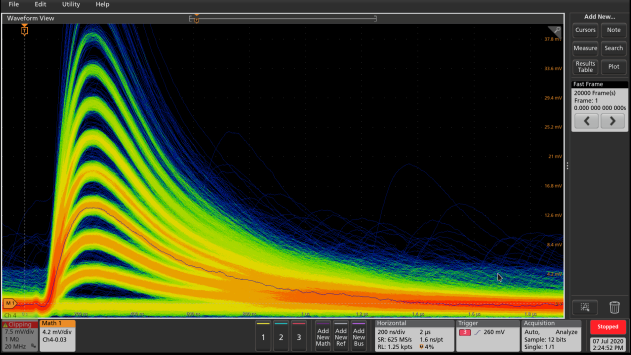
\includegraphics[scale=0.6]{3DesignPrinciples/32Tritium_detector/Several_SiPM_pulses.png}
\caption{Using persistence on the oscilloscope to show several pulses with different heights. Each height associated with a different number of  SiPM pixels lit at the same time.\label{fig:PulsesOfSiPM}}
\end{figure}

If the photon density to be detected is low enough, only one photon in each pixel are detected. Therefore, these pixels need to be very small\footnote{Pixel sizes for commercial SiPMs are $50$ or $75\mu\meter$ \cite{DataSheetHammamatsu_1_SiPM_50}, \cite{DataSheetHammamatsu_1_SiPM_75}}. When the photon density are high (several thousand of photons per event) two or more photons will be detected by the same pixel, generating an output signal equal to one detected photon. This effect produces a loss of linearity of the output signal. This effect is known as saturation and this is not important for the TRITIUM detector since its scintillating signals are futher away from producing it. %The experimental measurements of this effect, which have been done for our SiPMs, is shown in section \ref{sec:CharacterizationSiPM}. 

The SiPM can be modeled as the electric circuit shown in figure \ref{subfig:ElectricModelSiPM} in which, due to the charge distribution in the depletion zone, a capacitance are induced by the SiPM. This looks like as a reverse diode in parallel with a capacitor with a capacitance of $C_d$. When the pixel detects a photon, the capacitor are discharged, creating an output current.

Each of these pixels has a quenching resistance\footnote{The tipical valuer of this quenching resistance for commercial SiPMs is around $500~\kilo\Omega$}, $R_q$, in series that is used to stop the current produced when this pixel is fired. When the discharge is produced, a current flow throguth the resistance, reducing the reverse voltage seen by the diode to one below the breakdown voltage. Then, the current that flow throught the diode is stopped and the voltage seen by the diode is reset to the bias voltage. This pixel is ready to detect a new photon again. This behaviour is schematicaly shown in Figure \ref{subfig:HowSiPMworks}.

\begin{figure}
\centering
    \begin{subfigure}[b]{0.45\textwidth}
    \centering
    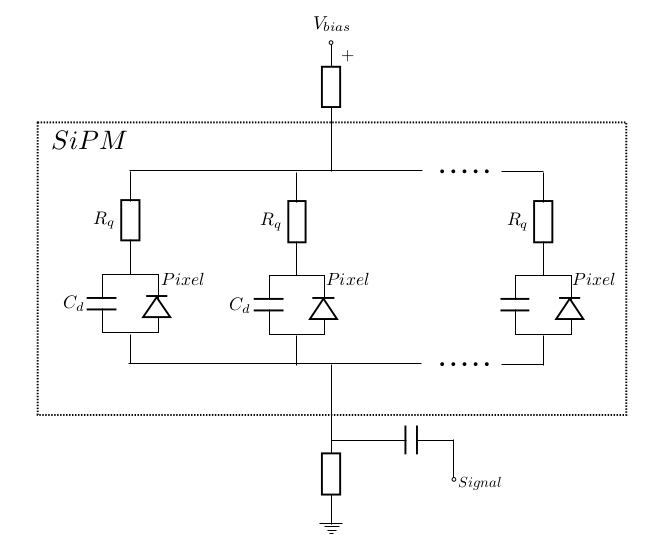
\includegraphics[width=\textwidth]{3DesignPrinciples/32Tritium_detector/SimpliestElectronicSchemeSiPM.png}  
    \caption{Photon Detection Efficiency, PDE.\label{subfig:ElectricModelSiPM}}
    \end{subfigure}
    \hfill
    \begin{subfigure}[b]{0.45\textwidth}
    \centering
    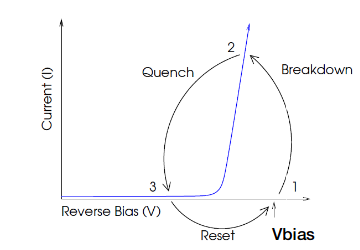
\includegraphics[width=\textwidth]{3DesignPrinciples/32Tritium_detector/How_a_quenching_resistence_in_a_SiPM_works.png}  
    \caption{Output current of a SiPM.\label{subfig:HowSiPMworks}}
    \end{subfigure}
 \caption{(Left) Electronic scheme of a SiPM and (right) output current of a SiPM as a function of the reverse voltage. It show that the quenching mechanism is essential for working with SiPMs~\cite{DataSheetSensL}.}
 \label{fig:ChenchingResistance}
\end{figure}

The recovery of the bias voltage seen by the SiPM after a photon detection is the characteristic in a RC circuit. 

\begin{equation}
V_bias(t)=V(t_0)\left(1-e^{-t/\tau} \right)
\label{RCCircuitBiasVoltage}
\end{equation}
where $\tau$ is the recovery time constant of the system, the value of which is $\tau=C_d \times R_q$ for RC circuits.

The capacitance $C_d$ and the quenching resistance $R_q$ are experimentally measured and the recovery time constant extrapolated from both. All of them are exhibited in section \ref{sec:CharacterizationSiPM}

SiPM gain is defined as the charge produced when a single pixel is fired. This can be measured experimentally from its Single Photon Spectrum, SPS, which is the spectrum obtained when the SiPM output signal is integred (charge) and histogrammed. The experimental measurement of the SPS and the extrapolation of the Gain is presented in section \ref{sec:CharacterizationSiPM}.

It has to be taken into account that the SiPM gain is highly dependent on temperature, which cannot be controlled with sufficient sensitivity (less than $1~\degree$) in the final placement of the TRITIUM monitor. Therefore, a gain stabilization method was developed to compensate for this effect. This method is detailed and tested in section \ref{sec:CharacterizationSiPM}

Explicar PDE

Explicar brevemente el tema de Afterpulses, Crosstolk y dark count rate y decir que ni esto ni el PDE se ha medido en este trabajo pero su medición es un tema pendiente.

The initial cadidate for TRITIUM project and the one which was characterized is the model S13360-1375 from Hamamatsu Photonics \cite{DataSheetHammamatsu_1_SiPM_1375} because this has interesting characteristics and properties, shown in Table \ref{tab:PropertiesOfSiPM1375}, such as high gain, low operating voltage, low afterpulses, crosstalk and dark counts than other SiPM models from Hamamatsu. This was later replaced by other model, S13360-6075 from Hamamatsu Photonics \cite{DataSheetHammamatsu_1_SiPM_75}. Its main difference is its higher active area ($6\times6~\mm^2$) which is achieved at the price of a higher dark count rate (typically 2 Mcps). In addition, commercial matrices are available covering a total size of $24\times24~\mm^2$.

%The candidate for TRITIUM project is S13360-6075 from Hamamatsu photonics \cite{DataSheetHammamatsu_1_SiPM_75} because its characteristics are the ones that best fit our objectives since this model has super low afterpulses, crosstalk and dark counts than other SiPM models from Hamamatsu. Its characteristics and properties are shown in Table \ref{tab:PropertiesOfSiPM75}. 

\begin{table}[htbp]
%%\centering.
\begin{center}
\begin{tabular}{|c|c|}
\hline
Parameter & Numerical value \\
\hline \hline \hline
Serie & $S13360$ \\ \hline
Model & $1375$ \\ \hline
Pixel Pitch ($\mu\meter$) & $75$ \\ \hline
Effective photosensitive area ($\mm^2$) & $1.3 \times 1.3$ \\ \hline
Number of pixels & $285$ \\ \hline
Fill factor & $82\%$ \\ \hline
Refractive index of windows material & $1.55$ \\ \hline
Operating temperature range ($\degree C$)& $[-20,60]$ \\ \hline
Spectral response range, $\lambda$ ($\nano\meter$) & $[320, 900]$ \\ \hline
Peak sensitivity wavelength, $\lambda_p$ ($\nano\meter$) & $450$ \\ \hline
PhotoDetection Efficiency, PDE, $\lambda=\lambda_p$ ($\%$) & $50$ \\ \hline
Dark counts, Typical/Maximum (kcps) & $90/270$ \\ \hline
Terminal capacitance, $C_t$ ($\pico\farad$) & $60$ \\ \hline
Gain, M, & $4 \cdot{} 10^6$ \\ \hline
Breakdown Voltage, $V_{BR}$ ($\volt$) & $53$ \\ \hline
Cross talk probability($\%$) & $7$ \\ \hline
Temperature coefficient $\Delta TV_{op}$ (m$\volt/\degree C$) & $54$ \\ \hline
\end{tabular}
\caption{Characteristics of SiPM S13360-1375 from Hamamatsu Photonics \cite{DataSheetHammamatsu_1_SiPM_1375}.}
\label{tab:PropertiesOfSiPM1375}
\end{center}
\end{table}

These values, provided by Hamamatsu photonics, are only approximate for a given element. Therefore, these parameters must be measured experimentally for each SiPM used because they can vary significatively even for SiPMs of the same model. The most important characteristics for the TRITIUM project are experimentaly measured and given in section \ref{sec:CharacterizationSiPM}. 

Although TRITIUM detector uses whole SiPM matrices, the caracterizations has been carried out at the level of a single SiPM to learn about the values of the SiPM parameters and to test the gain control method.
 
%The matrices selected are of the model "S13361-6050" from Hamamatsu, which consists of a $4\times 4$ SiPM matrix where the active area of each SiPM is $6\times 6~\mm$ \cite{DataSheetHammamatsu_array_SiPM_6050} or the model "S13361-3050" from Hamamatsu, which consists of a $8\times 8$ SiPM where the active area is $3\times 3~\mm$ \cite{DataSheetHammamatsu_array_SiPM_3050}. They are commercial matrices from Hamamatsu and the total active area that is covered is the same for both models, $24\times 24~\mm$ and it is approximatelly the same as the active area covered with the PMTs employed, described in the previous section. These matrices have a common bias voltage and ground for all SiPMs but a different output signal for each SiPM. 

%We hope to obtain better results with the 4x4 matrix for theoretical reasons which we will see in section \ref{sec:CharacterizationSiPM} like larger PDE, mainly due to a larger active area but it is something that we will have to verify with experimental measurements.